\section{问题一的模型建立与求解}

\subsection{控制方程与边界条件}
令 $T(r,t)$ 和 $C(r,t)$ 分别表示药材温度和干基含水率。问题一采用固定半径 $R_0=0.02\,\mathrm m$ 的一维径向模型：
\begin{equation}
 \rho c_p\frac{\partial T}{\partial t}=\frac1r\frac{\partial}{\partial r}\left(rk\frac{\partial T}{\partial r}\right),\qquad
 \frac{\partial C}{\partial t}=\frac1r\frac{\partial}{\partial r}\left(rD(C)\frac{\partial C}{\partial r}\right).
\end{equation}
中心满足 $T_r(0,t)=C_r(0,t)=0$，表面满足
\begin{equation}
 -kT_r(R_0,t)=h(T_s-T_\infty),\qquad -D(C_s)C_r(R_0,t)=k_m(C_s-C_e).
\end{equation}
其中 $T_\infty,C_e$ 来自附件 1 的分段线性插值，热物性取附录 2，$D(C)=7\times10^{-9}\exp(-0.89/C)$。连续介质模型用于描述内部温度和水分场的时空变化[\cite{ref2}]。

\subsection{环形有限体积离散}
将 $[0,R_0]$ 划分为 $N$ 个环形控制体，对每个控制体积分后，中心面面积为零，内部面通量由相邻单元共享，从而保留圆柱几何权重并保证离散通量守恒。对非线性水分扩散定义 Kirchhoff 积分势
\[
 K(C)=\int_0^C\exp(-0.89/s)\,\mathrm ds,
\]
则 $D(C)C_r=7\times10^{-9}K_r$。类似的积分变换可用于浓度依赖扩散通量的处理[\cite{ref4}]。最外半控制体与 Robin 条件联立，利用括区间 Brent 求根得到真实表面含水率，再计算表面通量。这样既避免直接平均低含水率下的扩散率，也不把表面状态误当作最外单元中心值。

\subsection{时间推进与结果}
空间离散后得到刚性常微分方程组，采用带稀疏结构的自适应 BDF 推进，在每个 60 s 环境节点分段积分，输出采样与内部步长分离。正式计算使用 $N=4096$、相对容差 $10^{-10}$、绝对容差 $10^{-11}$、最大步长 $10\,\mathrm s$。

\begin{figure}[H]
  \centering
  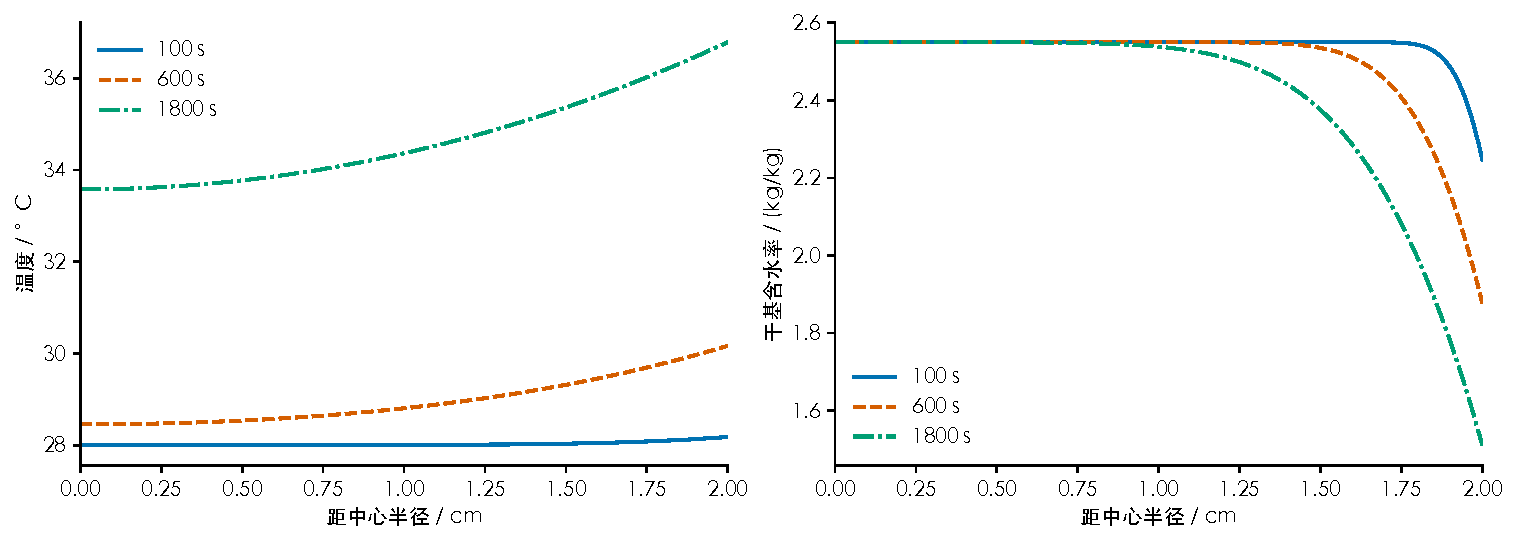
\includegraphics[width=0.82\textwidth]{../figures/q1/q1_profiles.pdf}
  \caption{问题一预热阶段温度与含水率径向剖面}
  \label{fig:q1profiles}
\end{figure}

\begin{table}[H]\centering\small
\caption{问题一预热阶段温度（$^\circ$C）}\label{tab:q1temp}
\resizebox{\textwidth}{!}{\begin{tabular}{rrrrrr}\toprule 时间/s & 0 cm & 0.5 cm & 1 cm & 1.5 cm & 2 cm\\\midrule
100&28.0001&28.0003&28.0040&28.0327&28.1801\\300&28.0408&28.0635&28.1514&28.3681&28.8489\\600&28.4533&28.5360&28.8039&29.3159&30.1652\\900&29.3243&29.4583&29.8755&30.6161&31.7304\\1200&30.5427&30.7098&31.2223&32.1126&33.4276\\1500&31.9957&32.1867&32.7660&33.7463&35.1203\\1800&33.5753&33.7720&34.3642&35.3621&36.7856\\\bottomrule\end{tabular}}\end{table}
\begin{table}[H]\centering\small
\caption{问题一预热阶段含水率（kg/kg）}\label{tab:q1moisture}
\resizebox{\textwidth}{!}{\begin{tabular}{rrrrrr}\toprule 时间/s & 0 cm & 0.5 cm & 1 cm & 1.5 cm & 2 cm\\\midrule
100&2.5500&2.5500&2.5500&2.5500&2.2470\\300&2.5500&2.5500&2.5500&2.5492&2.0508\\600&2.5500&2.5500&2.5500&2.5353&1.8770\\900&2.5500&2.5500&2.5497&2.5045&1.7547\\1200&2.5500&2.5500&2.5482&2.4646&1.6586\\1500&2.5500&2.5499&2.5445&2.4206&1.5787\\1800&2.5500&2.5497&2.5383&2.3755&1.5102\\\bottomrule\end{tabular}}\end{table}
表 1 和表 2 的原始数据分别见 \texttt{results/q1/table1.csv} 与 \texttt{results/q1/table2.csv}；图~\ref{fig:q1profiles}展示典型时刻的径向分布。

数值复核中，2048 到 4096 单元的工作簿网格最大变化为 $1.504\times10^{-7}\,\mathrm K$（温度）和 $2.851\times10^{-5}\,\mathrm{kg/kg}$（含水率）；收紧时间设置后的最大变化分别为 $1.537\times10^{-7}\,\mathrm K$ 和 $2.950\times10^{-9}\,\mathrm{kg/kg}$。独立圆柱热方程基准的最大温度偏差为 $1.804\times10^{-7}\,\mathrm K$，说明当前条件模型下离散实现稳定。
